\documentclass{article}
\usepackage[utf8]{inputenc}
\usepackage{float}
\usepackage{indentfirst}


\title{Exploration of Stevens’s Power Law}
\author{Justin Myerson and Michael Corace}

\usepackage{natbib}
\usepackage{geometry}
 \geometry{
 a4paper,
 total={170mm,257mm},
 left=20mm,
 top=20mm,
 }
\usepackage{graphicx}
\usepackage{multicol}
\setlength{\columnsep}{1cm}


\begin{document}

\maketitle

\begin{multicols}{2}

\section{Introduction}
Numerous experiments have been conducted to explore the different relationships of stimuli in regards to Stevens’s Power Law. With new technologies and visualization techniques, many aspects of modern visualizations have not been thoroughly explored. Our goal is to help define how human perception is affected by these stimuli. Static comparative brightness affects every visualization designer, as users of electronic displays can alter the brightness at will. Understanding how their users will perceive different levels of brightness could help inform visualization designers how they can better represent data along this channel. \citep{bauer2009does}\citep{heer2010crowdsourcing}\citep{rensink2000seeing}\par

Another common stimuli that has not been thoroughly explored is velocity. Animation is a popular tool amongst designers, but it has been determined to not be an effective way of communicating information. \cite{chevalier2014not}\cite{robertson2008effectiveness} Animation is, however, excellent at attracting attention. Human eyes are trained to be drawn to movement since birth, but how well humans can estimate this motion has not been fully studied in regard to computer animation. \cite{rensink2002change} We plan to abstract a single piece of animation, in this case the velocity, and test how accurately its magnitude is perceived. If there were to be an accurate description of how well people estimated different velocities of animation, it could open up a new visual channel to explore. Information could be encoded in visualizations in a new way, especially with the processing power of modern machines.\par 

A series of experiments will be used to determine how well the magnitude of change in these channels is perceived by our volunteers. We plan to conduct experiments involving line length and area to prove that our method of data collection is accurate in reference to the established Steven’s Exponents of these channels.

\section{Background}
Stevens's Power Law provides a good guideline for how people perceive stimuli magnitudes, but most of the studied stimuli are not applicable to modern-day computer-generated visualizations \cite{bolton2008modeling}. Through this project, we sought to remedy this by providing experimental results for 4 fundamental aspects of visualization: brightness, length, area, and velocity. From our results, we find that length and area require refinement from the original results proposed by Stevens, and assign exponents to brightness and velocity for the first time. \cite{bauer2009does}

\section{Design Rationale}
\begin{figure}[H]
    \centering
    
\includegraphics[width=\columnwidth]{Area}
    \caption{Area Test}
    \label{fig:Area}
\end{figure}

\begin{figure}[H]
    \centering
    
\includegraphics[width=\columnwidth]{Brightness}
    \caption{Brightness Test}
    \label{fig:Brightness}
\end{figure}

\begin{figure}[H]
    \centering
    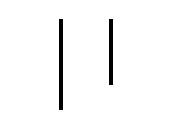
\includegraphics[width=\columnwidth]{Length}
    \caption{Length Test}
    \label{fig:Length}
\end{figure}

\begin{figure}[H]
    \centering
    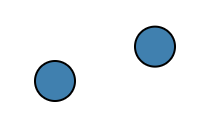
\includegraphics[width=\columnwidth]{Velocity}
    \caption{Velocity Test}
    \label{fig:Velocity}
\end{figure}

Above are 4 testing samples from our experiments. In each of the 4 versions, the participant is given the value of the item on the left as a reference, and asked to estimate the value of the item on the right. We adopted a scale of 1-100 for all 4 tests, so as to give the participants a consistent range to work with. For the velocity test, we chose a minimum duration from top to bottom of 1 second. Chevalier et al. note a minimum practical duration of .5 seconds, but we found this was too small in the relatively short trip from top to bottom in our visualization. \citep{chevalier2014not} Our focus was getting an accurate perception of the movement speed, and not finding the minimal speed necessary to track the circles accurately. 

\section{Experiments}
To conduct our experiments we had ten participants respond to ten tests for each type of visual channel, for a total of 40 tests per person. Each test was completely random so that we could limit the amount of additional effects that could impact the results. \cite{heer2010crowdsourcing} During the test a participant would see two shapes and would be shown the value ascribed to the shape on the left. This value represented the visual channel we were testing, whether it be velocity, brightness, area, or line length. To make it easier on the participant we scaled the values of all tests to only fall between 1 and 100. The participant would then be asked to enter what value (1-100) best represented the shape on the right, based on the given value. The four different visual channels were randomly cycled through until all 40 tests were completed, while each test displayed randomly selected Given and Test values. The procedure for this experiment was heavily influence by Stevens himself, who used a similar method when trying to measure how humans perceive the ratio of two audio samples. \citep{stevens1956direct}
\section{Analysis}
\begin{figure}[H]
    \centering
    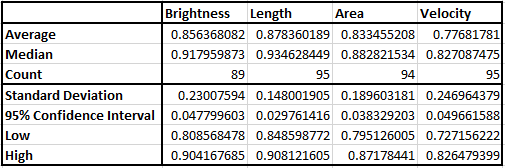
\includegraphics[width=\columnwidth]{Table}
    \caption{The results of the experiments.}
    \label{fig:Table}
\end{figure}

After gathering our experimental results, we performed some basic analysis on the data. First, we found the average and median of the data before deciding how best to calculate the final exponents. We then found standard deviation, and 95\%\ confidence intervals to give an idea of the distribution of the results. \cite{stevens1964concerning}\cite{teghtsoonian1971exponents}\par

\begin{figure}[H]
    \centering
    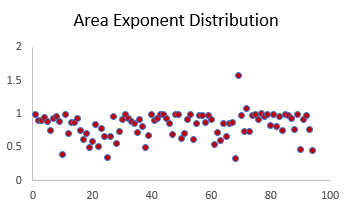
\includegraphics[width=\columnwidth]{AreaGraph}
    \caption{Area Exponent Distribution}
    \label{fig:AreaGraph}
\end{figure}

\begin{figure}[H]
    \centering
    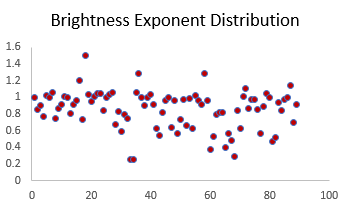
\includegraphics[width=\columnwidth]{BrightnessGraph}
    \caption{Brightness Exponent Distribution}
    \label{fig:BrightnessGraph}
\end{figure}

\begin{figure}[H]
    \centering
    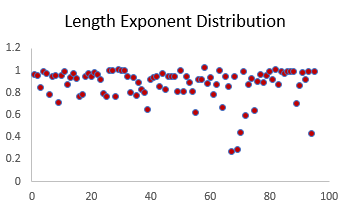
\includegraphics[width=\columnwidth]{LengthGraph}
    \caption{Length Exponent Distribution}
    \label{fig:LengthGraph}
\end{figure}

\begin{figure}[H]
    \centering
    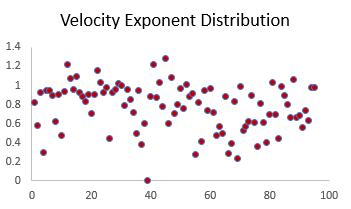
\includegraphics[width=\columnwidth]{VelocityGraph}
    \caption{Velocity Exponent Distribution}
    \label{fig:VelocityGraph}
\end{figure}

It's clear from the distribution graphs that the length and area results were much more consistent than the brightness and velocity, which is to be expected. This explains why so many of our values are outside of the 95\%\ confidence interval, and points to why the median is a better judgment of the overall results than the average. \cite{ericEJ982771} \par 

With this in mind, we calculate the following exponents for our 4 visualization types:
\begin{itemize}
    \item Area: .883 (Stevens calculated as .7)
    \item Brightness: .918
    \item Length: .935 (Stevens calculated as 1)
    \item Velocity: .827
\end{itemize}

\begin{figure}[H]
    \centering
    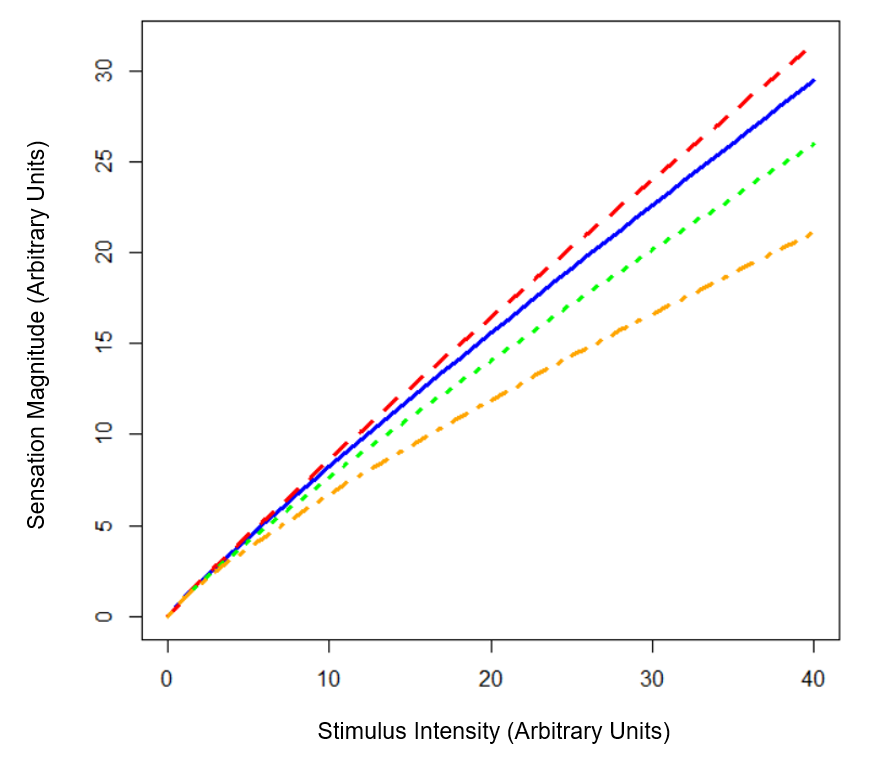
\includegraphics[width = \columnwidth]{exponents}
    \caption{Exponent values plotted onto a graph.}
    \label{fig:exponents}
\end{figure}

\section{Conclusion}
From the data we collected, we were able to draw some conclusions about how the different exponents relate to one another, and to the original values calculated by Stevens. The two values Stevens had previously calculated were Area and Line Length, and the exponents we received from our calculations were slightly off. The values still make sense because our results show that people under-estimate a change in area, and are fairly accurate with changes in linear length. \citep{bernasconi2016we} This is backed by numerous studies, including by Heer and Bostock as referenced prior. We submit that velocity the least accurate exponent is also accurate, as the task of estimating differences in magnitude of a moving object is more difficult than perceiving differences in line length or area. Stevens originally tested brightness using a single point of light flashing, and calculated the exponent of .7. Our revised method got a significantly higher exponent of .918, but we think this is reasonable since two projected squares on a screen will be easier to perceive than intermittent light flashes. 
\bibliographystyle{plain}
\bibliography{references}
\end{multicols}
\end{document}
